\documentclass{article}%
\usepackage[T1]{fontenc}%
\usepackage[utf8]{inputenc}%
\usepackage{lmodern}%
\usepackage{textcomp}%
\usepackage{lastpage}%
\usepackage[head=40pt,margin=0.5in,bottom=0.6in]{geometry}%
\usepackage{graphicx}%
%
\title{\textbf{Ortega Díaz: María Gabriela Chávez está involucrada en caso Andrade}}%
\author{El Nacional Web}%
\date{28/11/2018}%
%
\begin{document}%
\normalsize%
\maketitle%
\textbf{URL: }%
http://www.el{-}nacional.com/noticias/politica/ortega{-}diaz{-}maria{-}gabriela{-}chavez{-}esta{-}involucrada{-}caso{-}andrade\_261440\newline%
%
\textbf{Periodico: }%
EN, %
ID: %
261440, %
Seccion: %
Política\newline%
%
\textbf{Palabras Claves: }%
NO\_TIENE\newline%
%
\textbf{Derecho: }%
1.10, %
Otros Derechos: %
CONTEXTO, %
Sub Derechos: %
1.10.2\newline%
%
\textbf{EP: }%
NO\newline%
\newline%
%
\textbf{\textit{La hija del fallecido presidente Hugo Chávez presuntamente tiene dos investigaciones abiertas en el Ministerio Público por lavado de capitales y otros delitos}}%
\newline%
\newline%
%
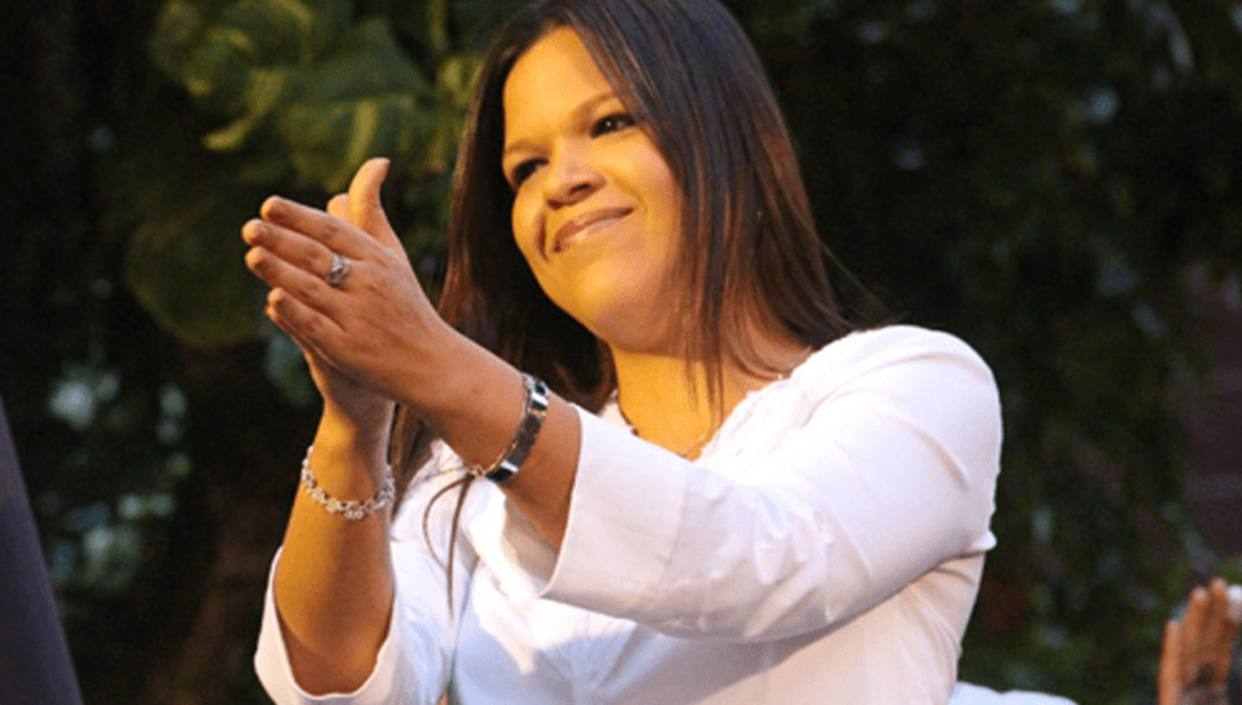
\includegraphics[width=300px]{182.jpg}%
\newline%
%
Luisa Ortega Díaz, fiscal general de la República en el exilio, señaló en una entrevista que María Gabriela Chávez, hija del presidente fallecido Hugo Chávez, está involucrada en el caso de Alejandro Andrade, quien fue acusado por la justicia norteamericana por lavado de capitales.%
\newline%
%
“EE UU tiene la pista tras de ella, porque el Ministerio Público venezolano hay dos investigaciones contra ella y contra Roberto Leiva, su pareja, por ese y otros delitos. Voy a dar el número de la investigación para quién usurpa el cargo le pida la privativa de libertad a María Gabriela Chávéz por lavado de dinero. Es MP4391762016”, dijo a~La Patilla.%
\newline%
%
Ortega Díaz expresó estar satisfecha con la sentencia dictada en contra de Andrade, que lo condena~a 10 años de prisión.%
\newline%
%
Indicó que el suceso fue investigado durante su gestión en el país y aseguró que colaboró con Estados Unidos al compartir información con las autoridades antes de exiliarse.%
\newline%
%
Con información de~La Patilla%
\newline%
%
\end{document}